\paragraph{General case}
Given two systems with degeneracy $g_1(N_1, U_1)$ and $g_2(N_2, U_2)$. $U_1+U_2 = U = \text{const}$ and $N_1=\text{const}$, $N_2=\text{const}$. We want to find maximal degeneracy:
$$\dv{U_1} g_1\cdot g_2 = \pdv{g_1}{U_1 } \cdot g_2 + \pdv{g_2}{U_2} \cdot \underbrace{\pdv{U_2}{U_1}}_{-1} \cdot g_1 = 0$$
$$\pdv{g_1}{U_1 }  \cdot \frac{1}{g_1} = \pdv{g_2}{U_2}  \cdot \frac{1}{g_2}$$
$$\pdv{\ln g_1}{U_1 }  = \pdv{\ln g_2}{U_2} $$
\paragraph{Temperature}
$$\frac{1}{T} = k_B + \pdv{U} \ln g$$
Define entropy (up to constant factor $k_B$)
$$\sigma = \ln g(N,U)$$
We also define
$$\frac{1}{\tau} = \frac{1}{k_B T} = \pdv{\sigma}{U}$$
If the system is continuous, we define number of states in some small interval as $\delta E$, then entropy is
$$\sigma = \ln \qty(g(N,U)\delta E)$$
and
$$\frac{1}{k_B T} = \pdv{\sigma}{U} = \pdv{U} \ln g + \underbrace{\pdv{U} \ln \delta E}_{\delta E = \text{const} \Rightarrow 0}$$
Also, define heat
$$\dd{Q} = \tau \dd{\sigma}$$
% \section{Thermodynamics}
\paragraph{Assumptions of thermodynamics}
\begin{enumerate}
	\item Heat is form of energy
	\item With high probability, the entropy of (non-equilibrium) closed system grows with time.
	\item When $\tau \to 0$, $\sigma\to0$ (there is one state).
\end{enumerate}
\subsection{Boltzmann distribution}
Suppose we divide a closed system into two parts: system and reservoir: 
\begin{center}
	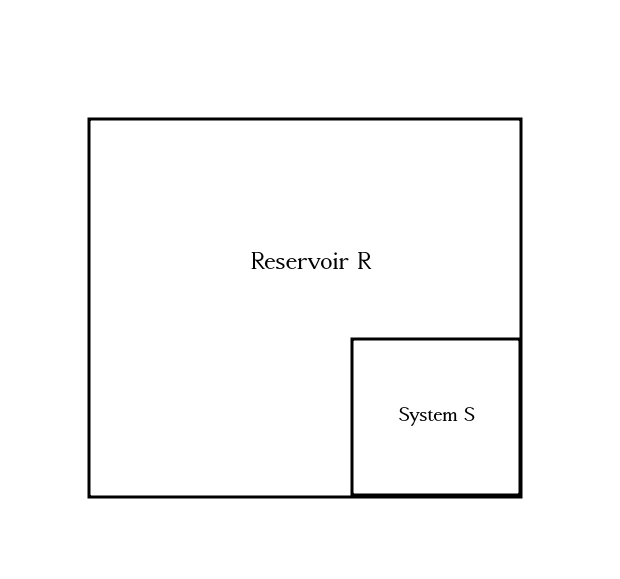
\includegraphics[width=0.5\linewidth]{./lect5/pic1.png}
\end{center}
What is probability that system $S$ will be in state which has energy $\epsilon$?
$$P_S(\epsilon)  \propto g_R(N,U_0 + \epsilon)$$
Where $U_0$ is total energy of reservoir + system. 
More precisely
$$P_S(\epsilon) = \frac{g_R(N,U_0 + \epsilon)}{g(U_0)}$$
For two states, ratio of probabilities is
\begin{align*}
\frac{P_S(\epsilon_1)}{P_S(\epsilon_2)} = \frac{g_R(N,U_0 - \epsilon_1)}{g_R(N,U_0 - \epsilon_2)} = e^{\sigma_R(U_0-\epsilon_1)-\sigma_R(U_0-\epsilon_2)}
\end{align*}
We assume that reservoir is much larger than system, i.e., $U_0 \gg \epsilon_0$:
$$\sigma_R(U_0 -\epsilon) = \sigma_R(U_0) - \pdv{\sigma_R}{U}\epsilon + \order{\epsilon^2} \approx  \sigma_R(U_0) - \frac{1}{\tau} \epsilon$$
Thus

$$\frac{P_S(\epsilon_1)}{P_S(\epsilon_2)} = \frac{g_R(N,U_0 \cdot \epsilon_1)}{g_R(N,U_0 \cdot \epsilon_2)} = e^{-\frac{1}{\tau} (\epsilon_1-\epsilon_2)} = \frac{ e^{-\frac{\epsilon_1}{\tau}}}{ e^{-\frac{\epsilon_2}{\tau}}}$$ 
If we want for any $\epsilon$
$$P_S(\epsilon) \propto e^{-\frac{\epsilon}{\tau}}$$

We want to define the partition function:
$$Z(\tau) = \sum_{\text{states}} e^{-\frac{\epsilon_{\text{state}}}{\tau}}$$
and thus we normalize
$$P_S(\epsilon) = \frac{e^{-\frac{\epsilon}{\tau}}}{Z(\tau)}$$
this is called Boltzmann factor.

Such system is called canonical ensemble.